\documentclass{article}
\usepackage{xcolor}
\usepackage{titleps}
\usepackage[letterpaper, margin=0.95in]{geometry}
\usepackage{url}
\usepackage{amsmath}
\usepackage{amssymb}
\usepackage{wrapfig}
\usepackage{float}
\usepackage{mathtools}
\usepackage{enumitem}
\usepackage{tabu}
\usepackage{parskip}
\usepackage{natbib}
\usepackage{listings}
\usepackage{tikz}
\usepackage{tikz-cd}
\usepackage{graphicx}
% \usepackage{quiver}

\newcommand{\xb}{\mathbf{x}}
\newcommand{\yb}{\mathbf{y}}
\newcommand{\wb}{\mathbf{w}}
\newcommand{\Xb}{\mathbf{X}}
\newcommand{\Yb}{\mathbf{Y}}
\newcommand{\tr}{^T}
\newcommand{\hb}{\mathbf{h}}
\newcommand{\Hb}{\mathbf{H}}

\DeclareFontShape{OT1}{cmtt}{bx}{n}{<5><6><7><8><9><10><10.95><12><14.4><17.28><20.74><24.88>cmttb10}{}


\usepackage{forest}

\usepackage{hyperref}
\usepackage[color=red]{todonotes}
\usepackage{forest}
\definecolor{light-yellow}{HTML}{FFE5CC}

\usepackage{cleveref}

\newpagestyle{ruled}
{\sethead{Berkeley CS 285}{Deep Reinforcement Learning, Decision Making, and Control}{Fall 2023}\headrule
  \setfoot{}{}{}}
\pagestyle{ruled}

\renewcommand\makeheadrule{\color{black}\rule[-.75\baselineskip]{\linewidth}{0.4pt}}
\renewcommand*\footnoterule{}

\begin{document}
\lstset{basicstyle = \ttfamily,columns=fullflexible,
backgroundcolor = \color{light-yellow}
}

\begin{centering}
    {\Large [SOLUTION TEMPLATE] Assignment 2: Policy Gradients} \\
    \vspace{.25cm}
    % \textbf{Due September 25, 11:59 pm} \\
    \textbf{Author: Jeremiah Chen} \\
\end{centering}

%%%%%%%%%%%%%%%%%%%%%%%%%%%%%%%%%%%%%%%%%%%%%%%%
% Policy Gradients
%%%%%%%%%%%%%%%%%%%%%%%%%%%%%%%%%%%%%%%%%%%%%%%%
\setcounter{section}{3}
\section{Policy Gradients}
\begin{itemize}
\item Create two graphs:
\begin{itemize}
\item In the first graph, compare the learning curves (average return vs. number of environment steps) for the experiments prefixed with \verb|cartpole|. (The small batch experiments.)
\item In the second graph, compare the learning curves for the experiments prefixed with \verb|cartpole_lb|. (The large batch experiments.)
\end{itemize}
\textbf{For all plots in this assignment, the $x$-axis should be number of environment steps, logged as} \verb|Train_EnvstepsSoFar| \textbf{(\textit{not} number of policy gradient iterations).}
\item Answer the following questions briefly: 
\begin{itemize}
\item Which value estimator has better performance without advantage normalization: the trajectory-centric one, or the one using reward-to-go?
\item Did advantage normalization help?
\item Did the batch size make an impact?
\end{itemize}
\item Provide the exact command line configurations (or \texttt{\#@params} settings in Colab) you used to run your experiments, including any parameters changed from their defaults.
\end{itemize}

\begin{figure}[H]
    \centering
    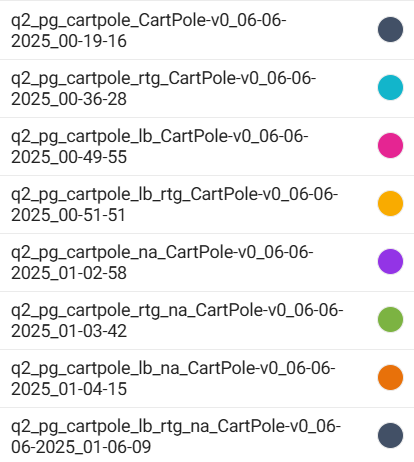
\includegraphics[width=0.35\textwidth]{img/q2_label.png}
    \caption{Labels for CartPole experiments}
    \label{fig:label_cartpole}
\end{figure}

\begin{figure}[H]
    \centering
    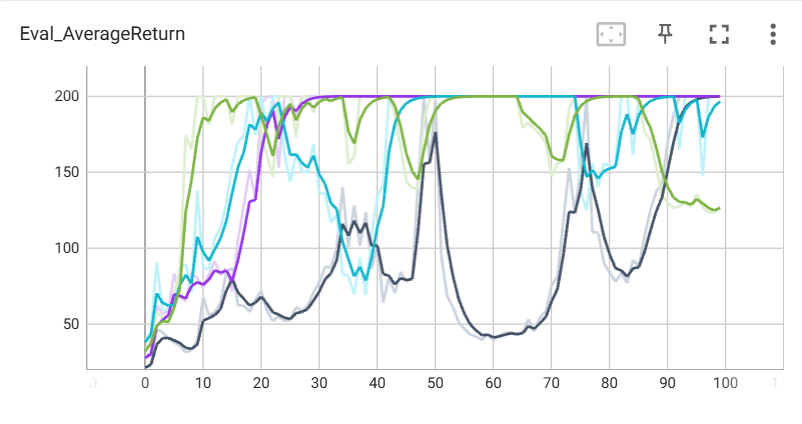
\includegraphics[width=0.8\textwidth]{img/cartpole_eval_avg_return.png}
    \caption{CartPole experiments}
    \label{fig:cartpole}
\end{figure}

\begin{figure}[H]
    \centering
    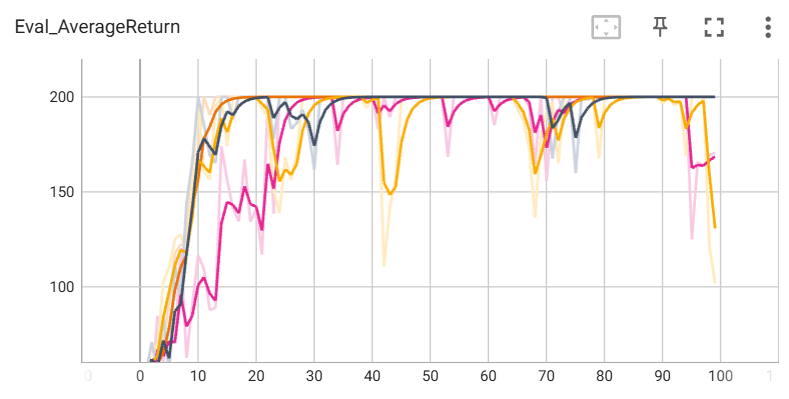
\includegraphics[width=0.8\textwidth]{img/cartpole_lb_eval_avg_return.png}
    \caption{CartPole experiments with large batch size}
    \label{fig:cartpole_lb}
\end{figure}

\textbf{Command line configurations:}
\begin{lstlisting}[language=bash]
# Small batch experiments
python cs285/scripts/run_hw2.py --env_name CartPole-v0 -n 100 -b 1000 \
--exp_name cartpole
python cs285/scripts/run_hw2.py --env_name CartPole-v0 -n 100 -b 1000 \
-rtg --exp_name cartpole_rtg
python cs285/scripts/run_hw2.py --env_name CartPole-v0 -n 100 -b 1000 \
-na --exp_name cartpole_na
python cs285/scripts/run_hw2.py --env_name CartPole-v0 -n 100 -b 1000 \
-rtg -na --exp_name cartpole_rtg_na
# Large batch experiments
python cs285/scripts/run_hw2.py --env_name CartPole-v0 -n 100 -b 4000 \
--exp_name cartpole_lb
python cs285/scripts/run_hw2.py --env_name CartPole-v0 -n 100 -b 4000 \
-rtg --exp_name cartpole_lb_rtg
python cs285/scripts/run_hw2.py --env_name CartPole-v0 -n 100 -b 4000 \
-na --exp_name cartpole_lb_na
python cs285/scripts/run_hw2.py --env_name CartPole-v0 -n 100 -b 4000 \
-rtg -na --exp_name cartpole_lb_rtg_na

\end{lstlisting}


According to the graphs, the reward-to-go estimator generally performs better than the trajectory-centric estimator, especially in the large batch experiments. Advantage normalization appears to help stabilize training, as seen in the smoother learning curves. The larger batch size leads to more stable updates and better performance, particularly in the large batch experiments.

The normalization of advantages helps to reduce variance in the policy gradient updates, leading to more stable learning.

The larger batch size does make a significant impact, as seen in the large batch experiments where the learning curves are smoother and the final performance is generally better compared to the small batch experiments.


%%%%%%%%%%%%%%%%%%%%%%%%%%%%%%%%%%%%%%%%%%%%%%%%
% Neural Network Baseline
%%%%%%%%%%%%%%%%%%%%%%%%%%%%%%%%%%%%%%%%%%%%%%%%
\newpage\section{Neural Network Baseline}
\begin{itemize}
    \item Plot a learning curve for the baseline loss.
    \item Plot a learning curve for the eval return. You should expect to achieve an average return over 300 for the baselined version.
    \item Run another experiment with a decreased number of baseline gradient steps (\verb|-bgs|) and/or baseline learning rate (\verb|-blr|). How does this affect (a) the baseline learning curve and (b) the performance of the policy?
    \item \textbf{Optional:} Add \verb|-na| back to see how much it improves things. Also, set \verb|video_log_freq 10|, then open TensorBoard and go to the ``Images'' tab to see some videos of your HalfCheetah walking along!
\end{itemize}

\begin{figure}[H]
    \centering
    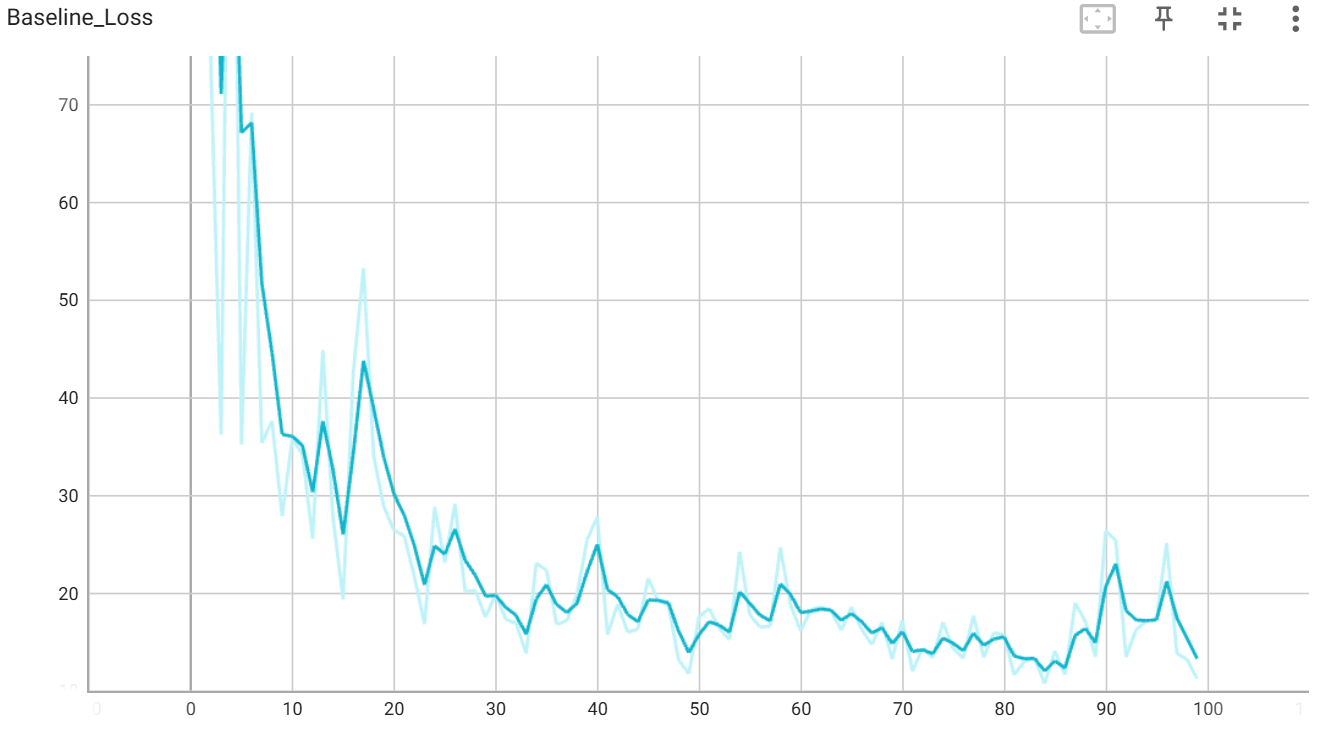
\includegraphics[width=0.7\textwidth]{img/HalfCheet_baseline_loss.png}
    \caption{Learning curve for the baseline loss}
    \label{fig:baseline_loss}
\end{figure}

\begin{figure}[H]
    \centering
    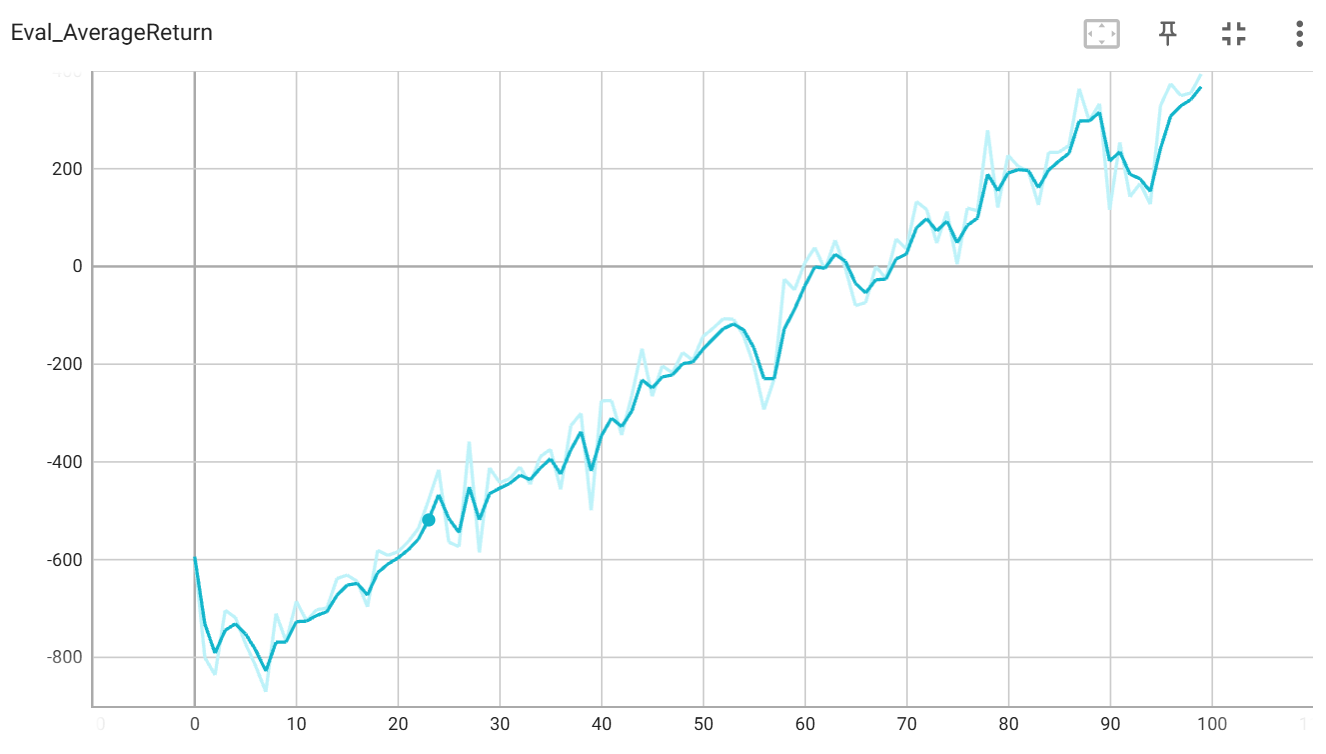
\includegraphics[width=0.7\textwidth]{img/HalfCheet_baseline_return.png}
    \caption{Learning curve for the baseline return}
    \label{fig:baseline_return}
\end{figure}
% \textbf{Default configurations:}
In the above experiments, we used the following default command line configurations:
\begin{lstlisting}[language=bash]
python cs285/scripts/run_hw2.py --env_name HalfCheetah-v4 \
-n 100 -b 5000 -rtg --discount 0.95 -lr 0.01 \
--use_baseline -blr 0.01 -bgs 5 --exp_name cheetah_baseline
\end{lstlisting}


\begin{figure}[H]
    \centering
    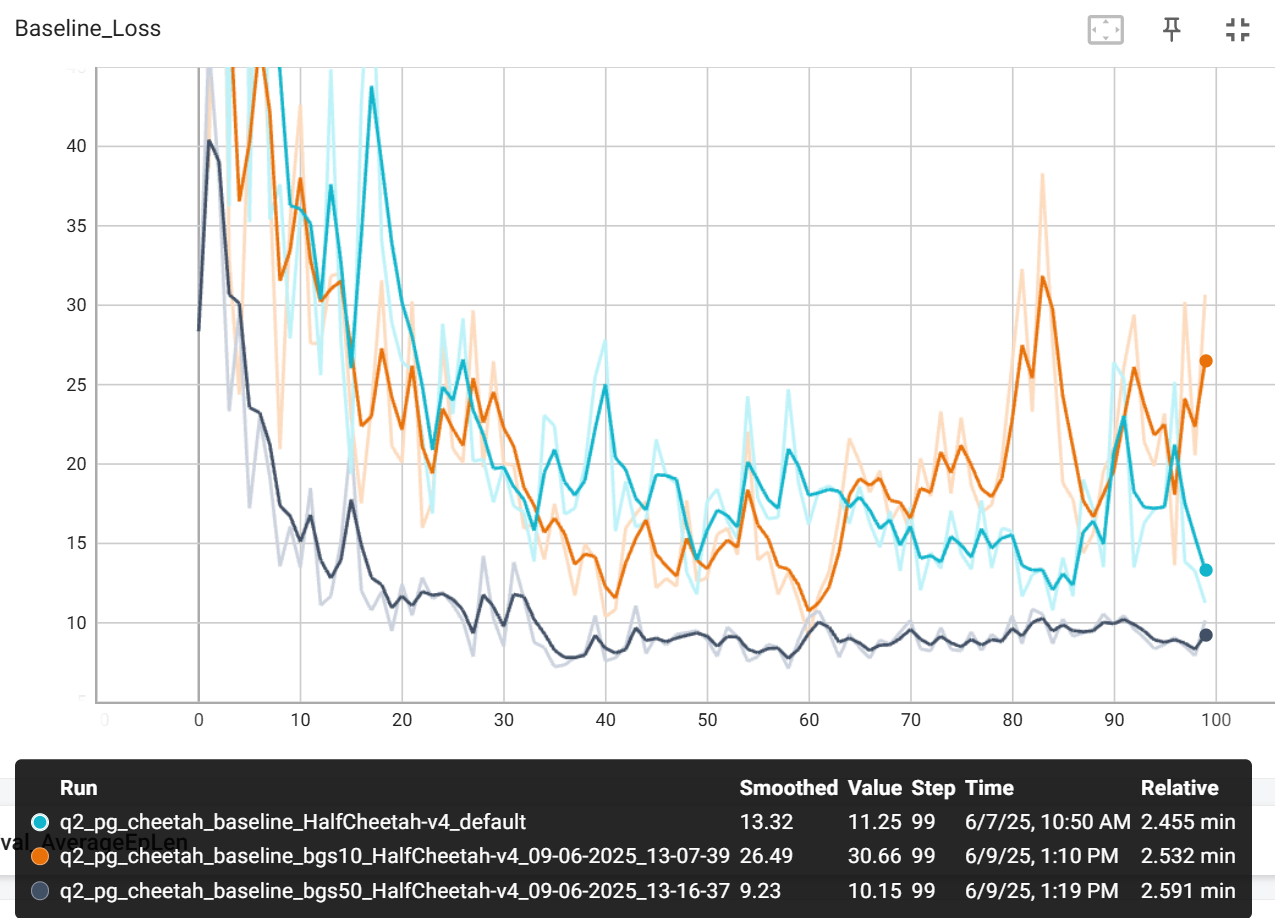
\includegraphics[width=0.7\textwidth]{img/HalfCheet_baseline_bgs_loss.png}
    \caption{Baseline loss in different baseline gradient steps}
    \label{fig:baseline_loss_bgs}
\end{figure}

\begin{figure}[H]
    \centering
    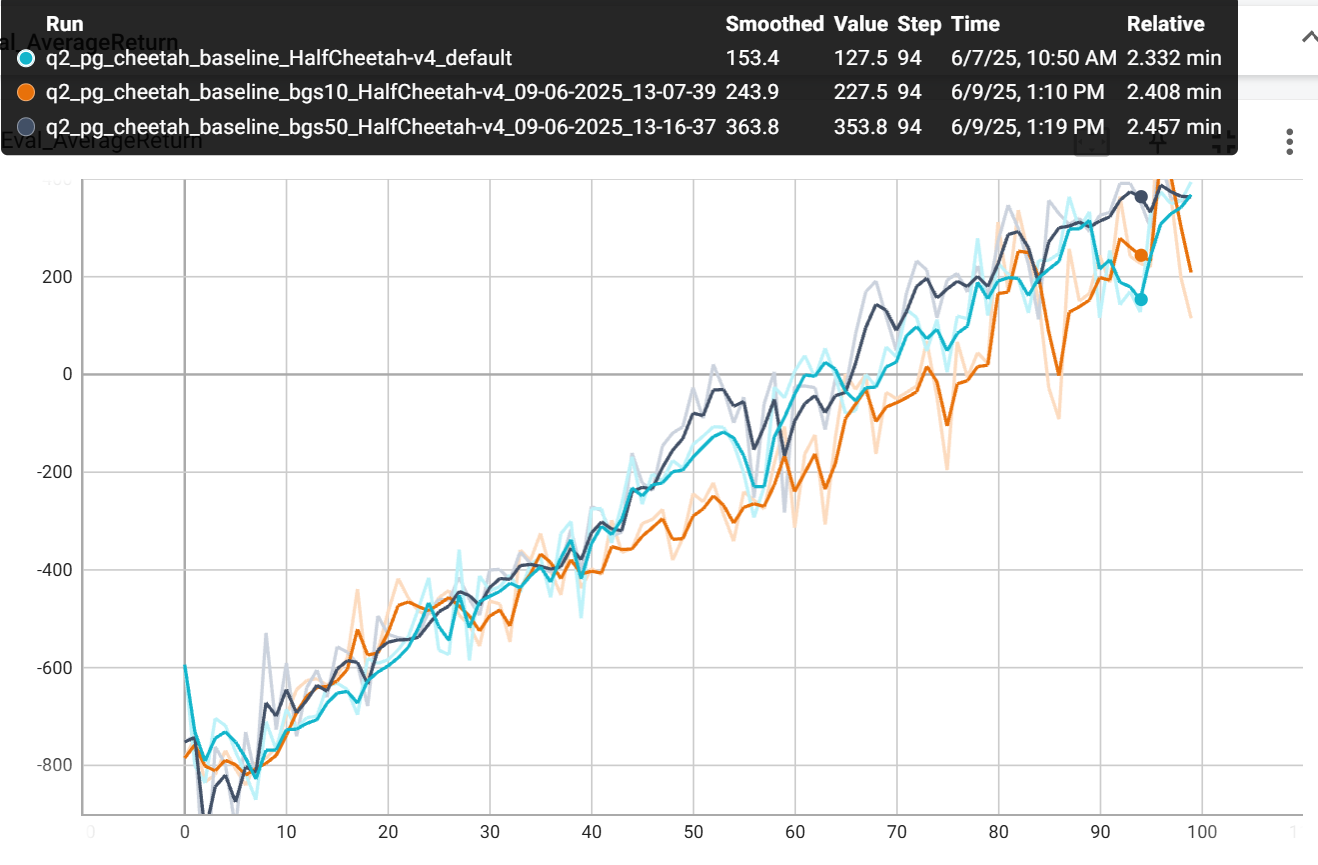
\includegraphics[width=0.7\textwidth]{img/HalfCheet_baseline_bgs_return.png}
    \caption{Baseline return in different baseline gradient steps}
    \label{fig:baseline_return_bgs}
\end{figure}

We try different baseline gradient steps $5$, $10$, and $50$.
The results show that increasing the number of baseline gradient steps leads to a more stable and smaller curve for the baseline loss,
and the performance of the policy improves as well, achieving a higher average return.

\begin{figure}[H]
    \centering
    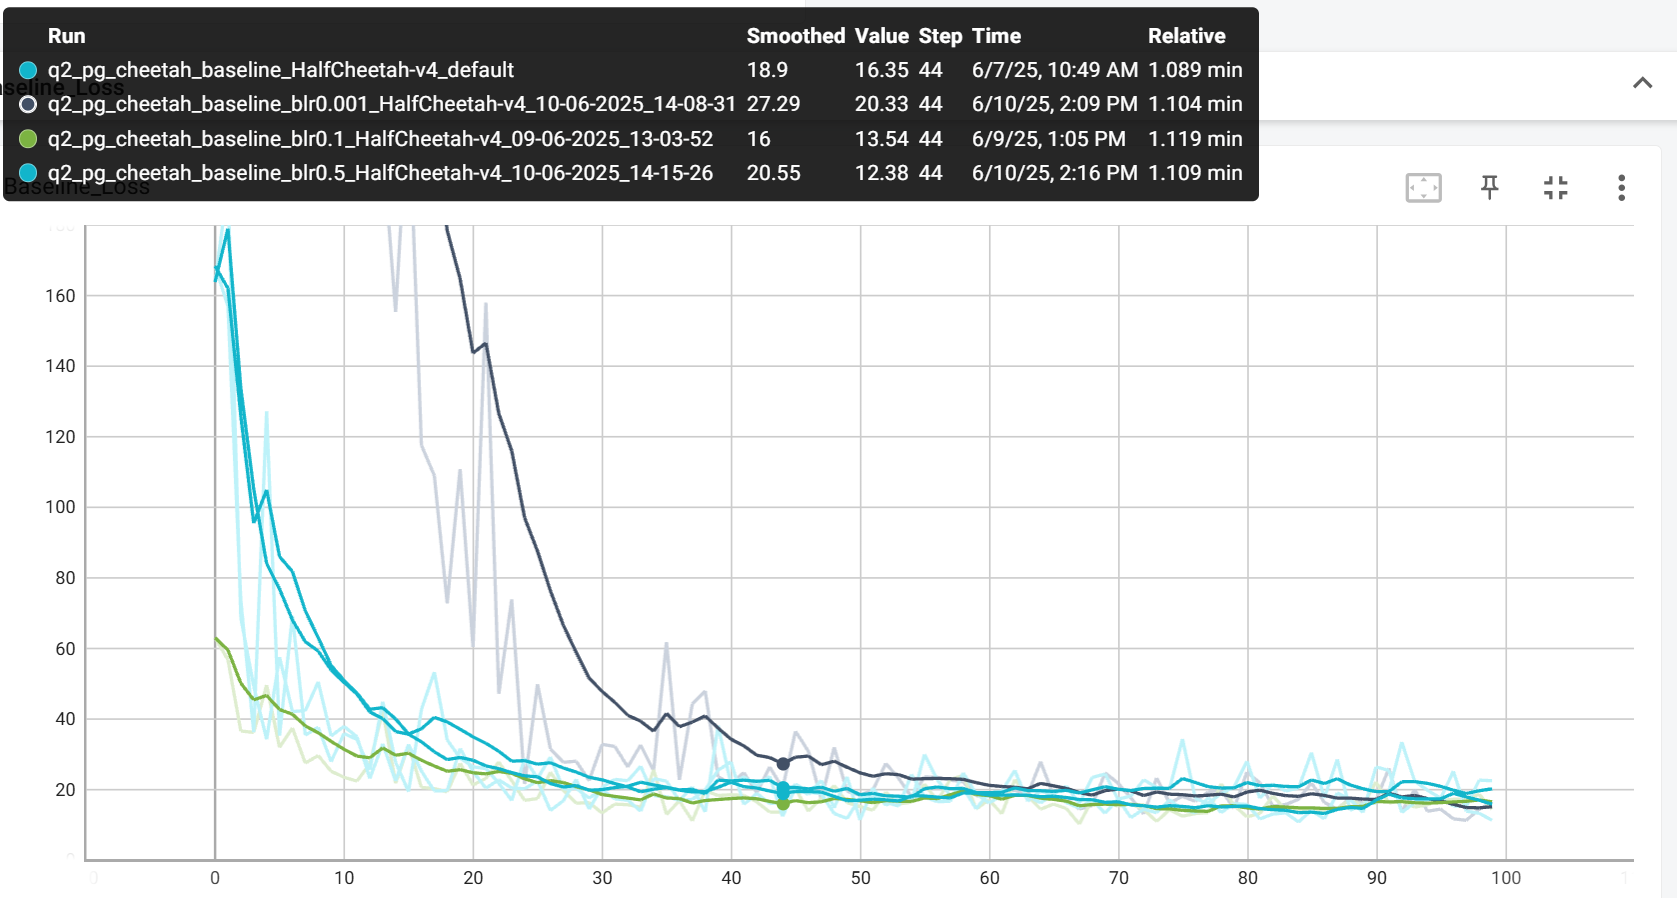
\includegraphics[width=0.7\textwidth]{img/HalfCheet_baseline_blr_loss.png}
    \caption{Baseline loss in different baseline learning rates}
    \label{fig:baseline_loss_blr}
\end{figure}

\begin{figure}[H]
    \centering
    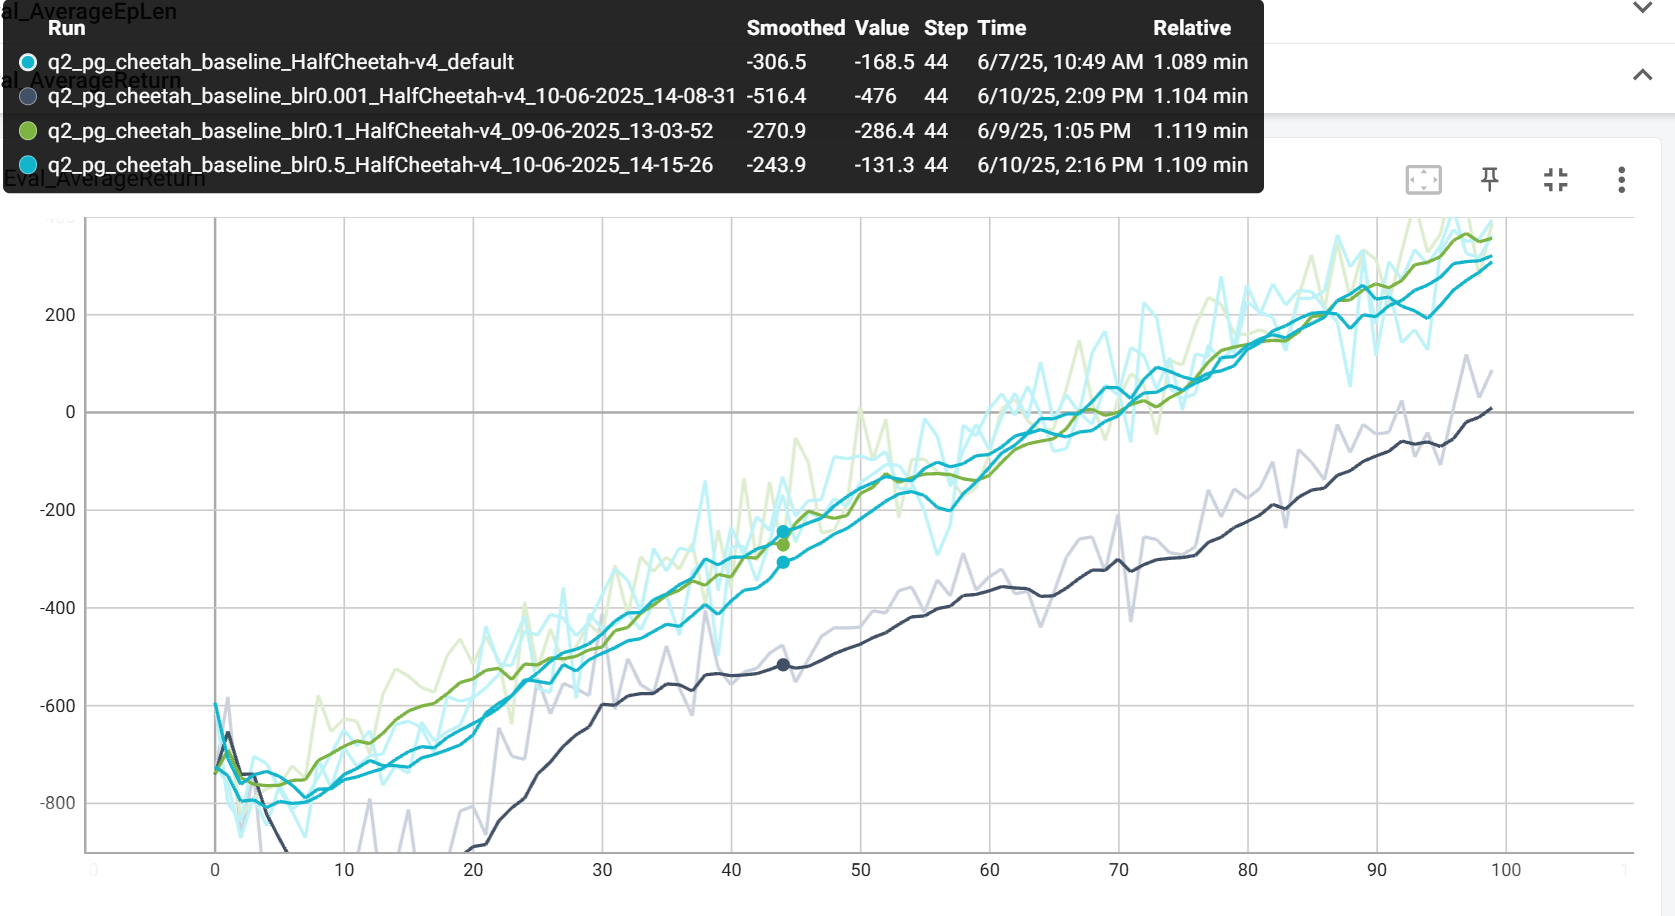
\includegraphics[width=0.7\textwidth]{img/HalfCheet_baseline_blr_return.png}
    \caption{Baseline return in different baseline learning rates}
    \label{fig:baseline_return_blr}
\end{figure}
We try different baseline learning rates $0.01$, $0.001$, $0.1$ and $0.5$.
We observe that slightly increasing the baseline learning rate leads to a more stable and smaller curve for the baseline loss, but the performance of the policy does not improve significantly.
Meanwhile, a too large baseline learning rate leads to a worse performance of the policy, achieving a lower average return.




\begin{figure}[H]
    \centering
    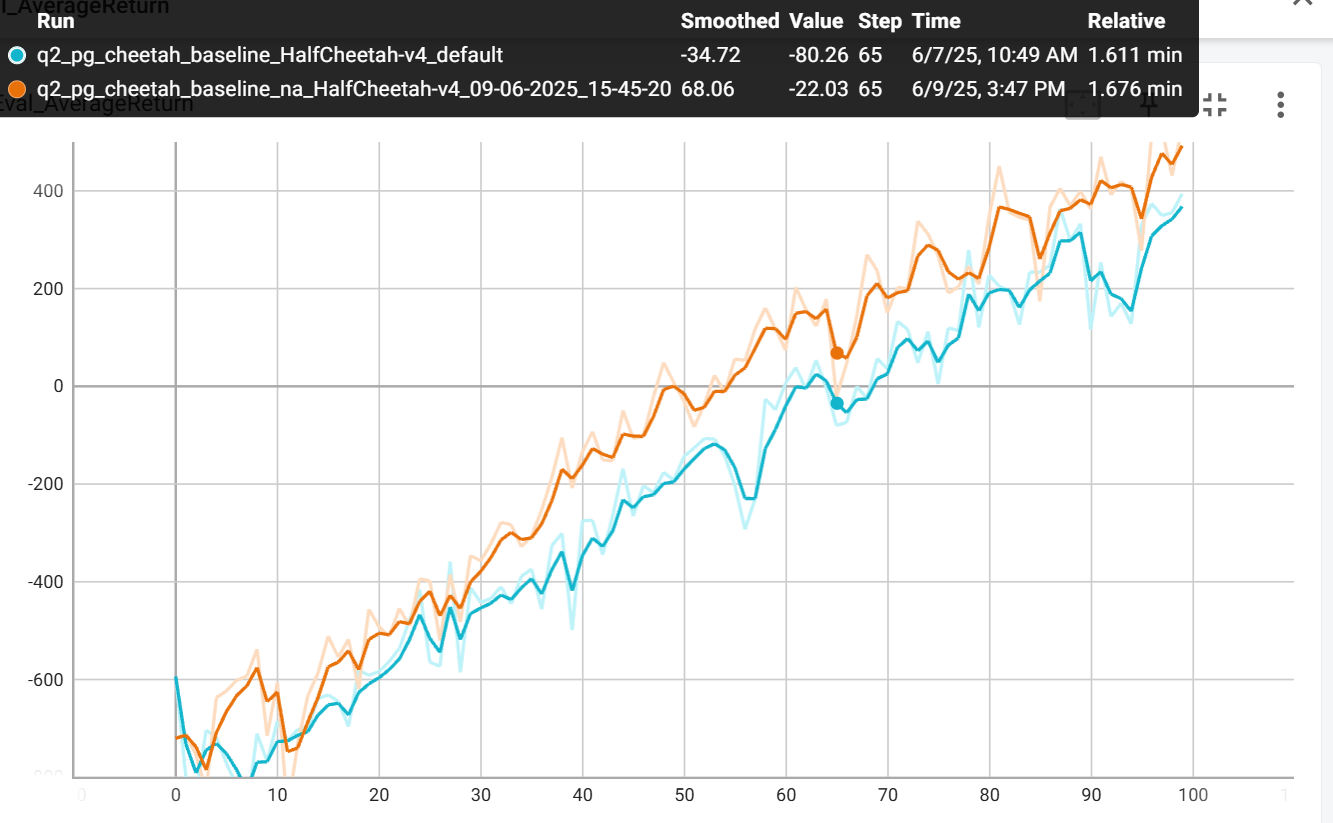
\includegraphics[width=0.7\textwidth]{img/HalfCheet_baseline_vs_na_return.png}
    \caption{Learning curve for the baseline return}
    \label{fig:baseline_vs_na_return}
\end{figure}
Compared to the deafult settings, adding \verb|-na| (normalization) leads to a more stable learning curve and better performance of the policy, achieving a higher average return. 

%%%%%%%%%%%%%%%%%%%%%%%%%%%%%%%%%%%%%%%%%%%%%%%%
% Generalized Advantage Estimation
%%%%%%%%%%%%%%%%%%%%%%%%%%%%%%%%%%%%%%%%%%%%%%%%
\newpage\section{Generalized Advantage Estimation}
\begin{itemize}
    \item Provide a single plot with the learning curves for the \verb|LunarLander-v2| experiments that you tried. Describe in words how $\lambda$ affected task performance. The run with the best performance should achieve an average score close to 200 (180+).
    \item Consider the parameter $\lambda$. What does $\lambda = 0$ correspond to? What about $\lambda = 1$? Relate this to the task performance in \verb|LunarLander-v2| in one or two sentences.
\end{itemize}

\begin{figure}[H]
    \centering
    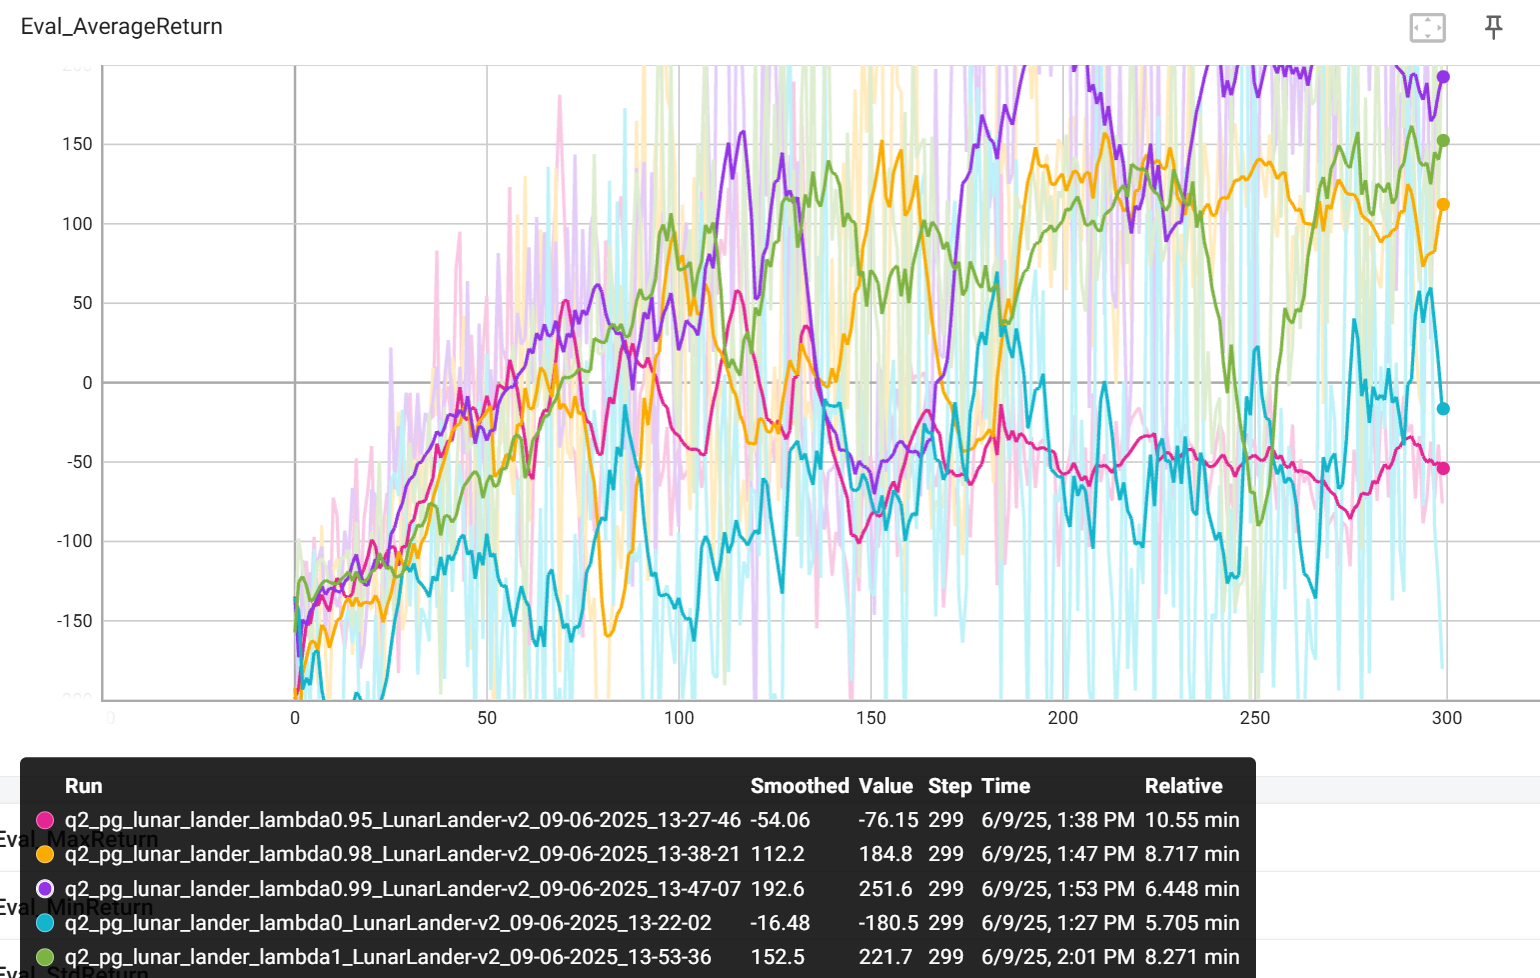
\includegraphics[width=0.7\textwidth]{img/GAE_return.png}
    \caption{GAE Learning curve for the baseline return}
    \label{fig:GAE_return}
\end{figure}

$\lambda = 0$: Corresponds to using only the immediate rewards at each timestep (ignoring future rewards), effectively disabling Generalized Advantage Estimation (GAE). This results in lower bias but higher variance in advantage estimation, which may lead to unstable training.

$\lambda = 1$: Corresponds to fully incorporating future rewards (similar to Monte Carlo methods), using complete GAE. This reduces variance but introduces higher bias, potentially slowing down convergence.

%%%%%%%%%%%%%%%%%%%%%%%%%%%%%%%%%%%%%%%%%%%%%%%%
% Hyperparameter Tuning
%%%%%%%%%%%%%%%%%%%%%%%%%%%%%%%%%%%%%%%%%%%%%%%%
\newpage\section{Hyperparameter Tuning}
\begin{enumerate}
    \item Provide a set of hyperparameters that achieve high return on \verb|InvertedPendulum-v4| in as few environment steps as possible.
    \item Show learning curves for the average returns with your hyperparameters and with the default settings, with environment steps on the $x$-axis. Returns should be averaged over 5 seeds.
\end{enumerate}



%%%%%%%%%%%%%%%%%%%%%%%%%%%%%%%%%%%%%%%%%%%%%%%%
% Humanoid
%%%%%%%%%%%%%%%%%%%%%%%%%%%%%%%%%%%%%%%%%%%%%%%%
\newpage\section{(Extra Credit) Humanoid}
\begin{enumerate}
    \item Plot a learning curve for the Humanoid-v4 environment. You should expect to achieve an average return of at least 600 by the end of training. Discuss what changes, if any, you made to complete this problem (for example: optimizations to the original code, hyperparameter changes, algorithmic changes).
\end{enumerate}

\begin{figure}[H]
    \centering
    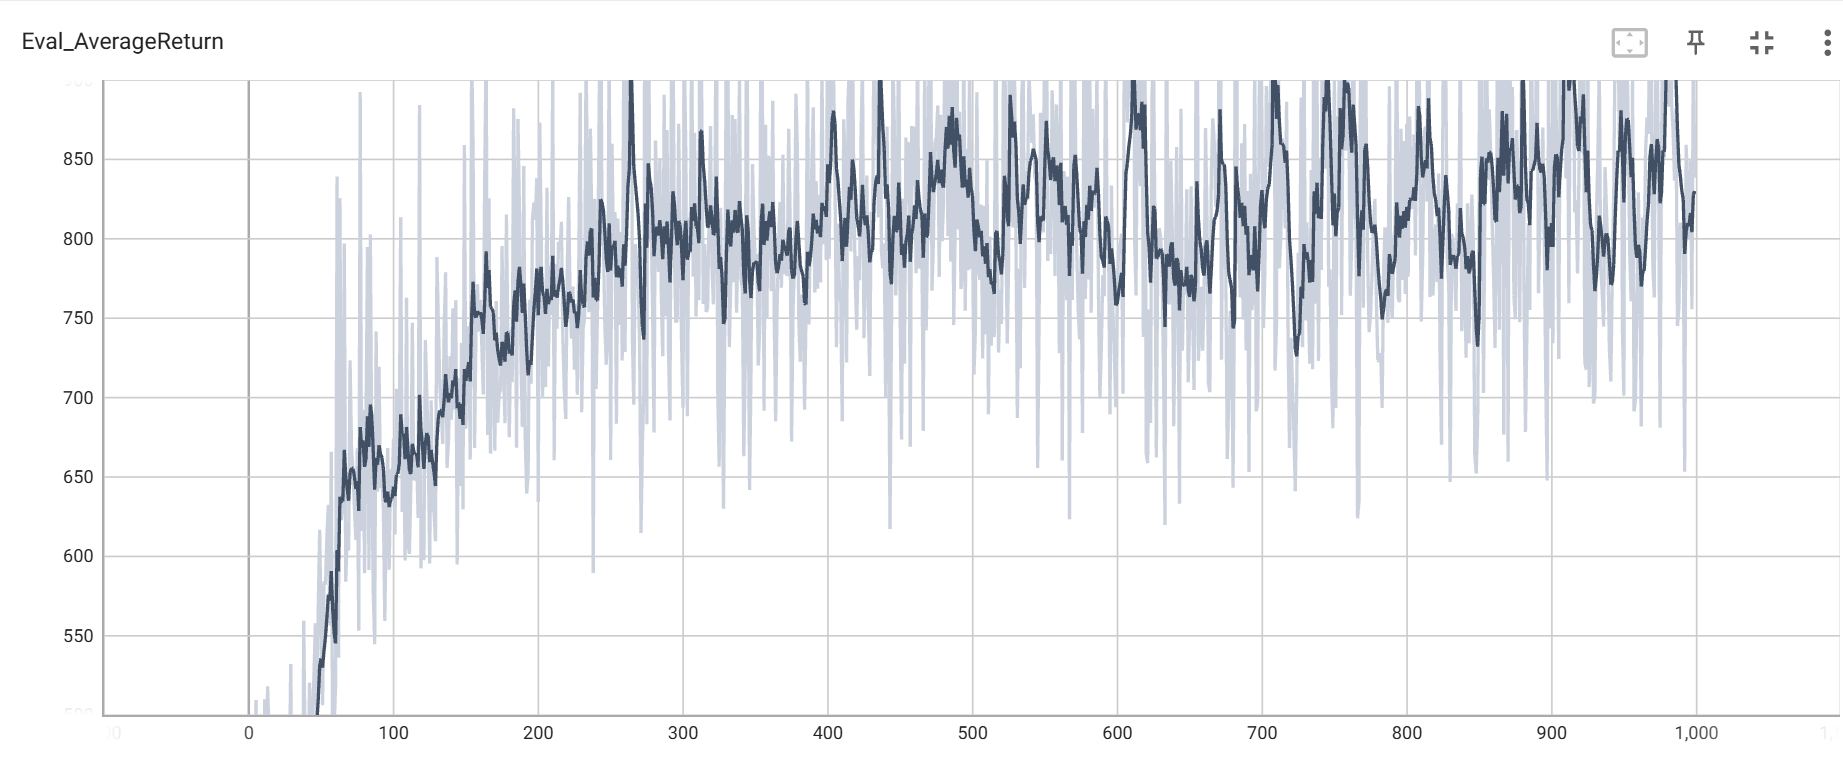
\includegraphics[width=0.8\textwidth]{img/Humanoid_Return.png}
    \caption{GAE Learning curve for the baseline return}
    \label{fig:Humanoid_return}
\end{figure}

%%%%%%%%%%%%%%%%%%%%%%%%%%%%%%%%%%%%%%%%%%%%%%%%
% Analysis
%%%%%%%%%%%%%%%%%%%%%%%%%%%%%%%%%%%%%%%%%%%%%%%%
\newpage\section{Analysis}
\label{sec:analysis}
Consider the following infinite-horizon MDP:
% https://q.uiver.app/#q=WzAsMixbMCwwLCJzIl0sWzAsMSwic19GIl0sWzAsMSwiYV8yIl1d
\[\begin{tikzcd}
	s_1 & {s_F}
	\arrow["{a_2}", from=1-1, to=1-2]
    \arrow["{a_1}", loop left, from=1-1, to=1-1]
\end{tikzcd}\]
\newcommand{\Rmax}[0]{R_{\textrm{max}}}
\newcommand{\E}[0]{\mathbb{E}}
\newcommand{\var}[0]{\textrm{Var}}
\crefname{question}{part}{parts}
\Crefname{question}{Part}{Parts}
\newcommand\question[1][]{\item\refstepcounter{subsection}\label[question]{#1}}

At each step, the agent stays in state $s_1$ and receives reward 1 if it takes action $a_1$, and receives reward 0 and terminates the episode otherwise.
Parametrize the policy as stationary (not dependent on time) with a single parameter:
\[\pi_\theta(a_1|s_1) = \theta, \pi_\theta(a_2|s_1) = 1-\theta\]

\begin{enumerate}
\question[sec:analysis1] Applying policy gradients
\begin{enumerate}
    \item Use policy gradients to compute the gradient of the expected return $R(\tau)$ with respect to the parameter $\theta$. \textbf{Do not use discounting.}

    \textbf{Hint}: to compute $\sum_{k=1}^\infty k\alpha^{k-1}$, you can write:
    \[\sum_{k=1}^\infty k\alpha^{k-1} = \sum_{k=1}^\infty \frac{d}{d\alpha}\alpha^k = \frac{d}{d\alpha}\sum_{k=1}^\infty\alpha^k\]

    \textbf{Solution:}

        $$
        \nabla J(\theta) = \nabla_{\theta} \left( \sum_{\tau} \pi_{\theta}(\tau) r(\tau) \right) = \sum_{\tau} \pi_{\theta}(\tau) \cdot \nabla_{\theta} \log \pi_{\theta}(\tau) \cdot r(\tau)
        $$

        Notice that $\pi_{\theta}(\tau) = \theta^k (1 - \theta)$ and $r(\tau) = k$.

        $$
        \begin{aligned}
        \nabla J(\theta) 
        &= \nabla_{\theta} \left( \sum_{\tau} \pi_{\theta}(\tau) r(\tau) \right) \\
        &= \sum_{\tau} \pi_{\theta}(\tau) \cdot \nabla_{\theta} \log \pi_{\theta}(\tau) \cdot r(\tau) \\
        % &= \sum_{k=1}^{\infty} \theta^k (1 - \theta) \cdot \nabla_{\theta} \log (\theta^k (1 - \theta)) \cdot k \\
        &= \sum_{k=1}^{\infty} \theta^k (1 - \theta) \left( \sum_{t=0}^{k} \nabla_{\theta} \log \pi_{\theta}(a_t | s_t) \right) \cdot k \\
        &= \sum_{k=1}^{\infty} \theta^k (1 - \theta) \left( \sum_{t=0}^{k-1} \frac{1}{\theta} + \frac{1}{1 - \theta} \right) \cdot k \\
        &= \sum_{k=1}^{\infty} \theta^k (1 - \theta) \left( k \theta^{k-1} - (k+1) \theta^k \right) \cdot \frac{1}{\theta^k (1 - \theta)} \cdot k \\
        &= \sum_{k=1}^{\infty} \left( k^2 \theta^{k-1} - k(k+1) \theta^k \right) \\
        &= \sum_{k=1}^{\infty} \left( k^2 \theta^{k-1} - (k+1)^2 \theta^k \right) + \sum_{k=1}^{\infty} (k+1) \theta^k \\
        &= 1 + \lim_{k \to \infty} (k+1) \theta^k + \frac{\theta}{(1-\theta)^2} + \theta \cdot \frac{1}{1-\theta} \\
        &= \frac{(1-\theta)^2 + \theta (1-\theta) + \theta}{(1-\theta)^2} \\
        &= \frac{1}{(1-\theta)^2}
        \end{aligned}
        $$
        

    \item \label{exact_gradient} Compute the expected return of the policy $\E_{\tau \sim \pi_\theta} R(\tau)$ directly. Compute the gradient of this expression with respect to $\theta$ and verify that this matches the policy gradient.
    
    \textbf{Solution:}
    
    $$
    \begin{aligned}
    \mathbb{E}_{\pi_{\theta}} R(\tau) &= \sum_{k=1}^{\infty} (k-1) \theta^{k-1} (1-\theta) \\
    &= \sum_{k=1}^{\infty} k \cdot \theta^k (1-\theta) \\
    &= \theta (1-\theta) \frac{d}{d\theta} \sum_{k=0}^{\infty} \theta^k \\
    &= \theta (1-\theta) \frac{d}{d\theta} \frac{1}{1-\theta} \\
    &= \theta (1-\theta) \cdot \frac{1}{(1-\theta)^2} = \frac{\theta}{1-\theta}
    \end{aligned}
    $$

    Verification:
    $$
    \nabla_{\theta} \mathbb{E}_{\pi_{\theta}} R(\tau) = \frac{1}{(1-\theta)^2}
    $$

    The results match the answer in part (a)

\end{enumerate}
\newpage
\question[sec:analysis2] Compute the variance of the policy gradient in closed form and describe the properties of the variance with respect to $\theta$. For what value(s) of $\theta$ is variance minimal? Maximal? (Once you have an exact expression for the variance you can eyeball the min/max).

\textbf{Hint:}  Once you have it expressed as a sum of terms $P(\theta)/Q(\theta)$ where $P$ and $Q$ are polynomials, you can use a symbolic computing program (Mathematica, SymPy, etc) to simplify to a single rational expression.

\textbf{Solution:}
    $$
    \begin{aligned}
    \text{Var}_{\pi_{\theta}} \left( \nabla_{\theta} J(\theta) \right) 
    = \mathbb{E}_{\pi_{\theta}} \left[ \left( \nabla_{\theta} \log \pi_{\theta}(\tau) \cdot r(\tau) \right)^2 \right] - \left( \nabla_{\theta} J(\theta) \right)^2 
    \end{aligned}
    $$

    $$
    \begin{aligned}
    \mathbb{E}_{\pi_{\theta}} \left[ \left( \nabla_{\theta} \log \pi_{\theta}(\tau) \cdot r(\tau) \right)^2 \right]
    &= \sum_{k=1}^{\infty} \theta^k (1-\theta) \cdot \left( \nabla_{\theta} \log (\theta^k (1-\theta)) \cdot k \right)^2 \\
    &= \sum_{k=1}^{\infty} \theta^k (1-\theta) \cdot k^2 \left( \frac{k \theta^{k-1} (k+1) \theta^k}{\theta^k (1-\theta)} \right)^2 \\
    &= \sum_{k=1}^{\infty} \theta^k (1-\theta) \cdot k^2 \left( \frac{k}{\theta} - \frac{1}{1-\theta} \right)^2 \\
    &= \frac{4\theta^2 + 9\theta + 1}{(\theta-1)^4 \cdot \theta}
    \end{aligned}
    $$

    $$
    \begin{aligned}
    \text{Var}_{\pi_{\theta}} \left( \nabla_{\theta} J(\theta) \right) &= \frac{4\theta^2 + 9\theta + 1}{(\theta-1)^4 \cdot \theta} - \frac{1}{(1-\theta)^4} \\
    &= \frac{4\theta^2 + 8\theta + 1}{(\theta-1)^4 \cdot \theta}
    \end{aligned}
    $$

    \begin{figure}[H]
    \centering
    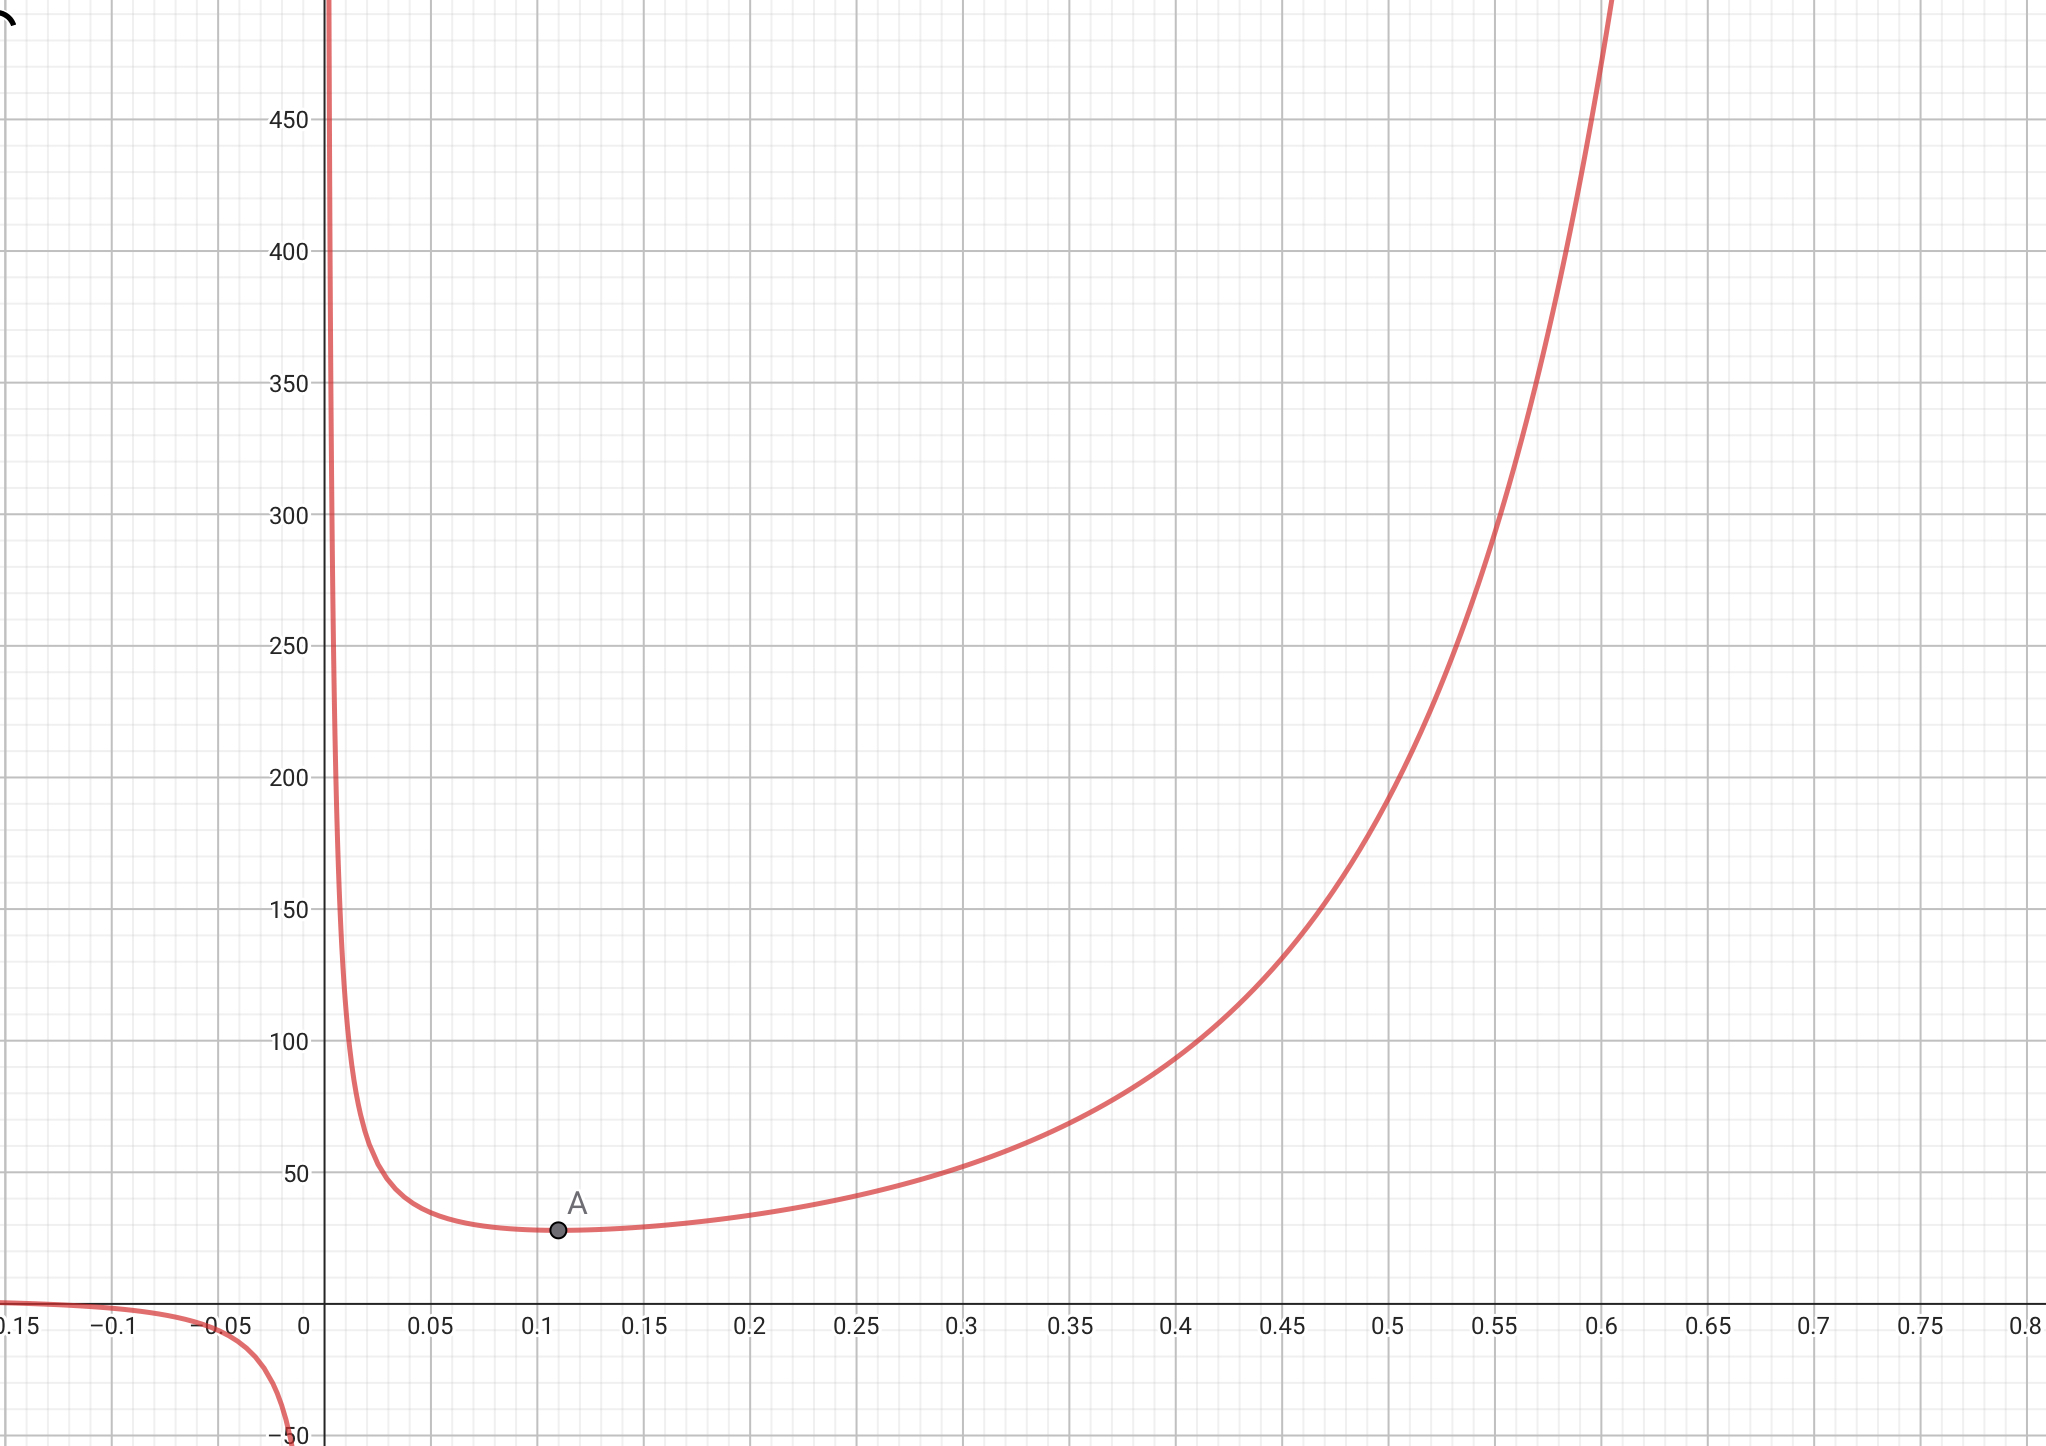
\includegraphics[width=0.7\textwidth]{img/PG_variance.jpg}
    \caption{Variance of the policy gradient}
    \label{fig:PG_variance}
    \end{figure}

    when $\theta = 0.1098822586019$, the variance is minimal, which is approximately $27.9411449358296$.

    And when $\theta = 0$ or $\theta = 1$, the variance is maximal, which is infinity.


\newpage
\question[sec:analysis3] Apply return-to-go as an advantage estimator.
\begin{enumerate}
    \item Write the modified policy gradient and confirm that it is unbiased.
    
    \textbf{Solution:}
    $$
    \begin{aligned}
    J(\theta) &= \sum_{k=1}^{\infty} \theta^k (1-\theta) \left( \sum_{t=0}^{k-1} \left( \frac{1}{\theta} \cdot (k-t) + \frac{1}{1-\theta} \cdot 0 \right) \right) \\
    &= \sum_{k=1}^{\infty} \theta^k (1-\theta) \cdot \frac{1}{\theta} \cdot \frac{k(k+1)}{2} \\
    &= \frac{1}{(1-\theta)^2}
    \end{aligned}
    $$

    \item Compute the variance of the return-to-go policy gradient and plot it on $[0, 1]$ alongside the variance of the original estimator.

    \textbf{Solution:}
    $$
    \begin{aligned}
    \text{Var}(\nabla J(\theta)) &= \mathbb{E}_{\pi_{\theta}} \left( \frac{1}{\theta^2} \cdot \frac{k^2 (k+1)^2}{4} \right) - \frac{1}{(1-\theta)^4} \\
    &= \sum_{k=0}^{\infty} \theta^k (1-\theta) \cdot \frac{1}{\theta^2} \cdot \frac{k^2 (k+1)^2}{4} - \frac{1}{(1-\theta)^4} \\
    &= \frac{\theta^2 + 4\theta + 1}{(\theta-1)^4 \cdot \theta} - \frac{1}{(1-\theta)^4} = \frac{(\theta+1)^2}{(\theta-1)^4 \cdot \theta}
    \end{aligned}
    $$

    \begin{figure}[H]
    \centering
    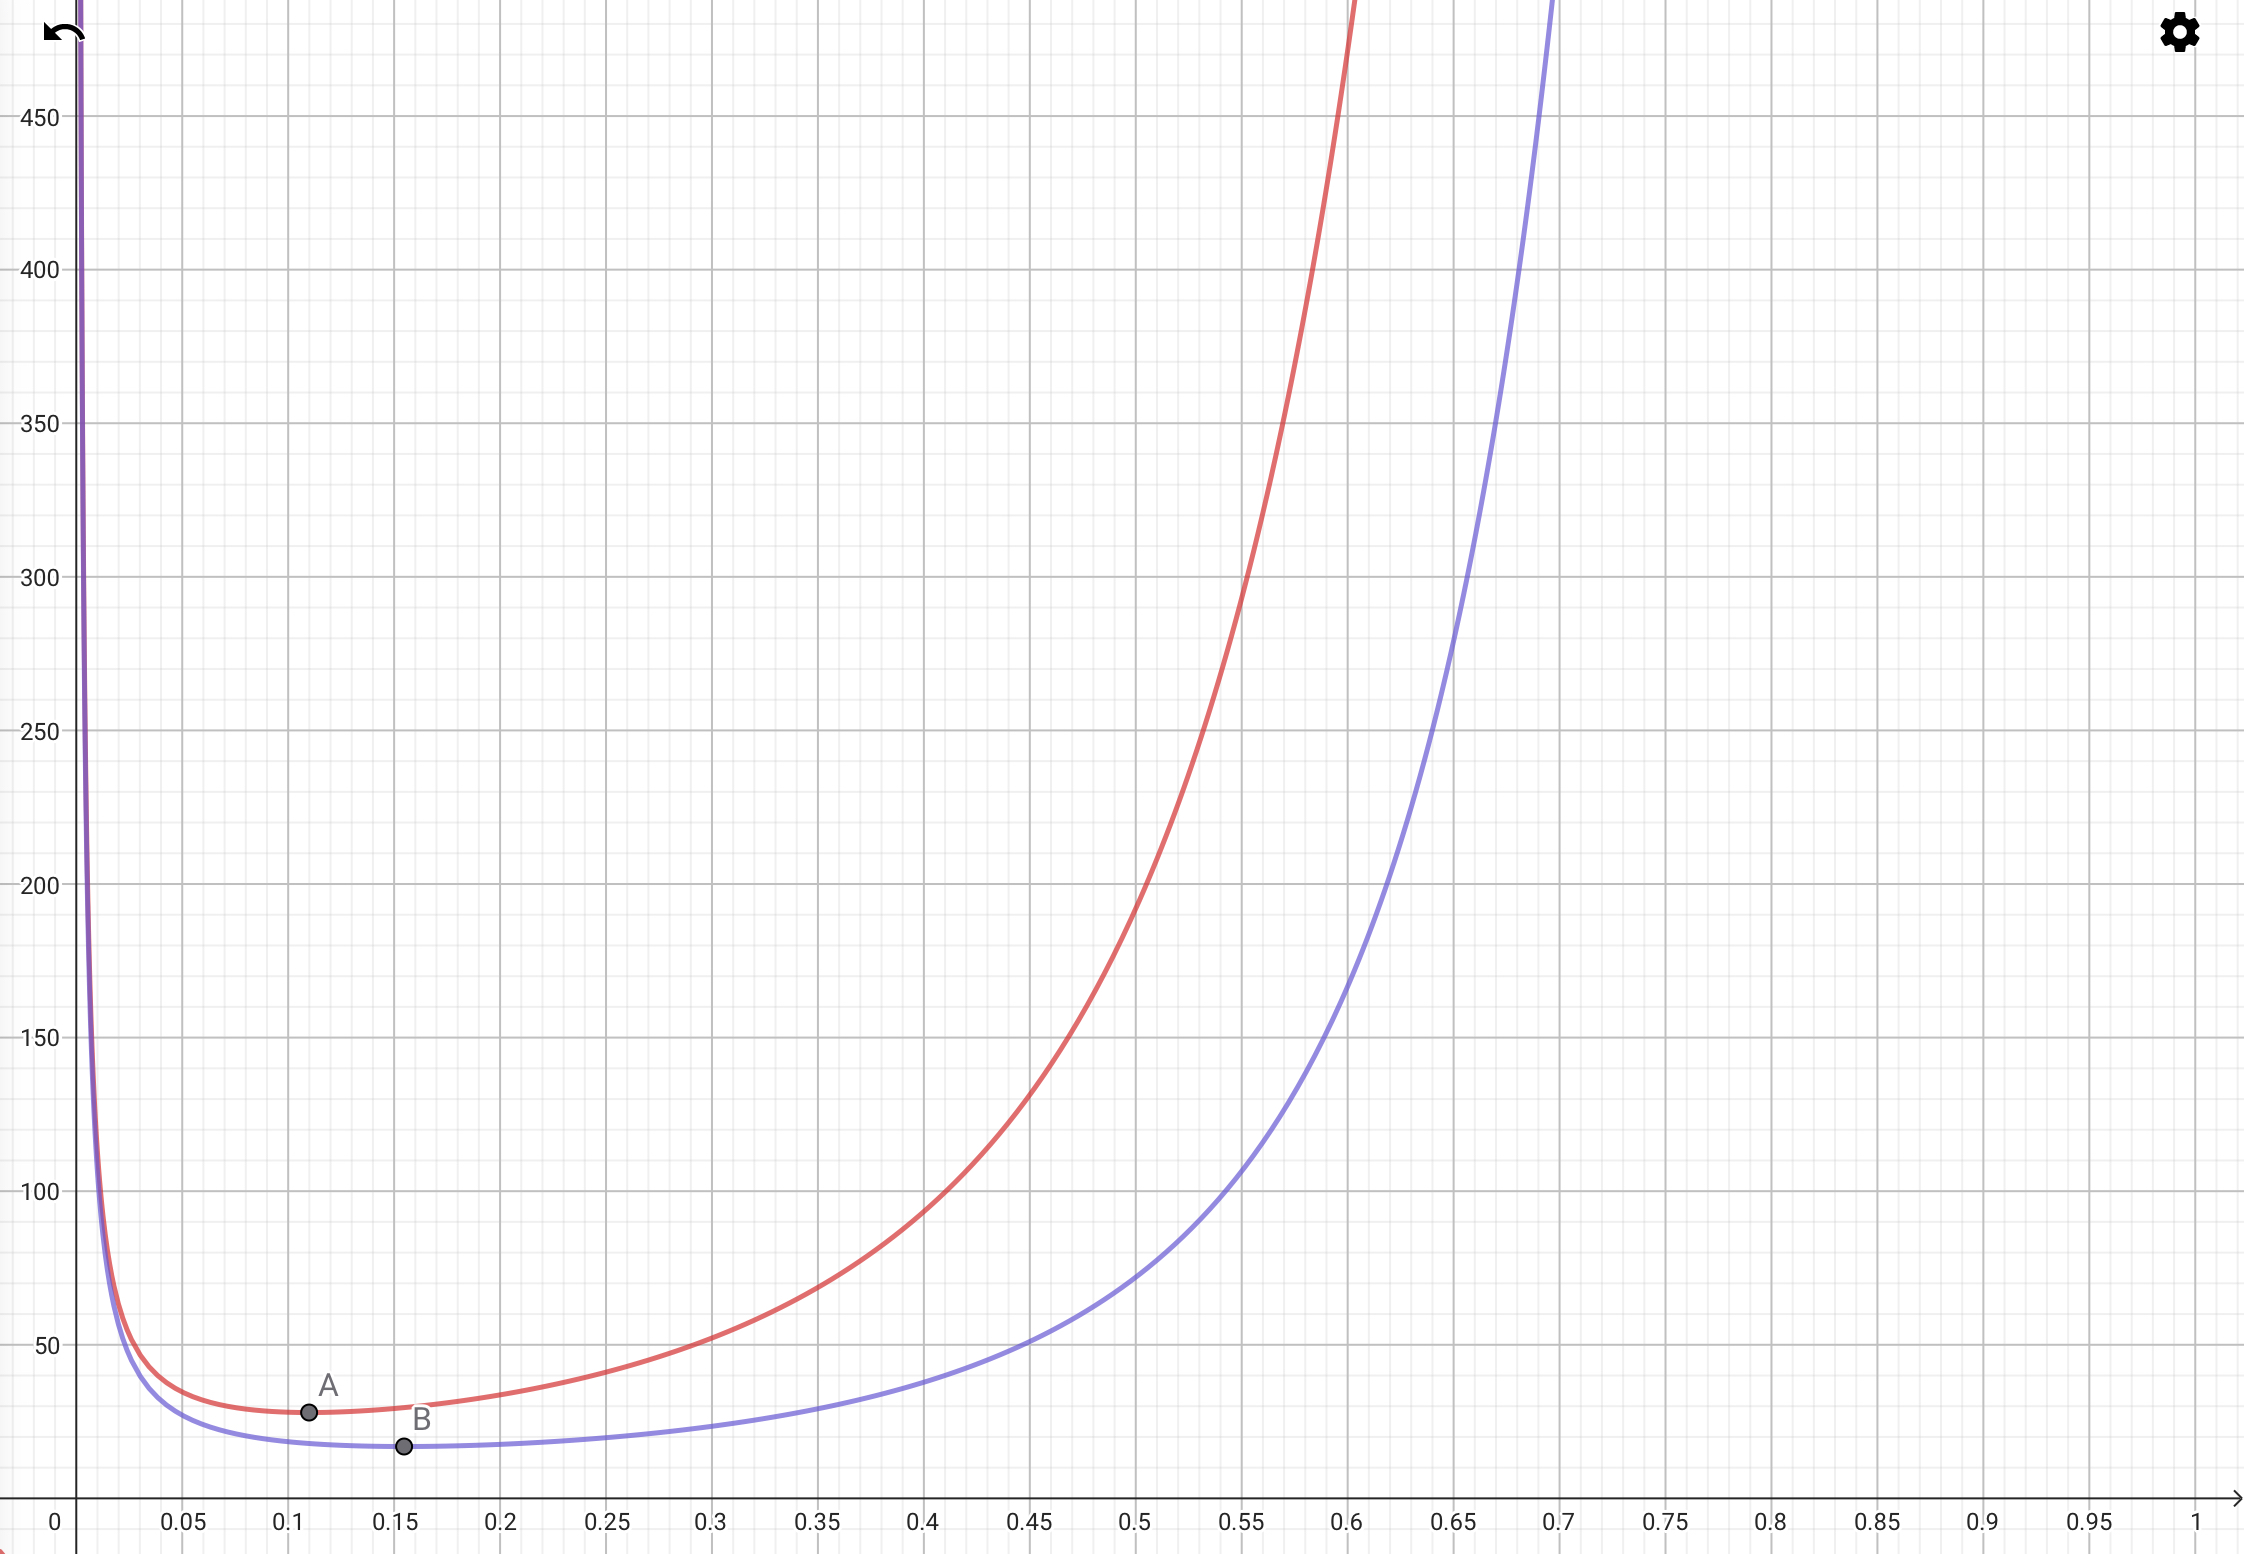
\includegraphics[width=0.7\textwidth]{img/PG_rtg_variance.jpg}
    \caption{Variance of retrun-to-go policy}
    \label{fig:PG_rtg_variance}
    \end{figure}

\end{enumerate}
\newpage
\question[sec:analysis4] Consider a finite-horizon $H$-step MDP with sparse reward:
% https://q.uiver.app/#q=WzAsNixbMCwwLCJzXzEiXSxbMSwwLCJzXzIiXSxbMiwwLCJzXzMiXSxbMiwxLCJzX0YiXSxbMywwLCJcXGRvdHMiXSxbNCwwLCJzX0giXSxbMCwxLCJhXzEiXSxbMSwyLCJhXzEiXSxbMCwzLCJhXzIiLDJdLFsyLDQsImFfMSJdLFs0LDVdLFsxLDMsImFfMiJdLFsyLDMsImFfMiIsMV0sWzQsMywiYV8yIiwxXV0=
\[\begin{tikzcd}
	{s_1} & {s_2} & {s_3} & \dots & {s_H} \\
	&& {s_F}
	\arrow["{a_1}", from=1-1, to=1-2]
	\arrow["{a_1}", from=1-2, to=1-3]
	\arrow["{a_2}"', from=1-1, to=2-3]
	\arrow["{a_1}", from=1-3, to=1-4]
	\arrow[from=1-4, to=1-5]
	\arrow["{a_2}", from=1-2, to=2-3]
	\arrow["{a_2}"{description}, from=1-3, to=2-3]
	\arrow["{a_2}"{description}, from=1-4, to=2-3]
\end{tikzcd}\]

The agent receives reward $\Rmax$ if it arrives at $s_H$ and reward $0$ if it arrives at $s_F$ (a terminal state). In other words, the return for a trajectory $\tau$ is given by:
\[R(\tau) = \begin{cases}1 & \tau \textrm{ ends at } s_H \\ 0 & \tau \textrm{ ends at } s_F \end{cases}\]
Using the same policy parametrization as above, consider off-policy policy gradients via importance sampling. Assume we want to compute policy gradients for a policy $\pi_\theta$ with samples drawn from $\pi_{\theta'}$.
\begin{enumerate}
    \item Write the policy gradient with importance sampling.
    
    \textbf{Solution:}
    $$
    \begin{aligned}
    \nabla_{\theta} J(\theta)
    &= \mathbb{E}_{x \sim p_{\theta}(x)} \left[ \frac{p_{\theta}(x)}{p_{\theta'}(x)} \nabla_{\theta} \log \pi_{\theta}(x) r(x) \right] \\
    &= \theta'^{H-1} \cdot \frac{\theta^{H-1}}{\theta'^{H-1}} \cdot \sum_{t=1}^{H-1} \nabla_{\theta} \log \pi_{\theta} \log (a_t | s_t) \\
    &= \theta^{H-1} \cdot \frac{H-1}{\theta} \\
    &= \theta^{H-2} \cdot (H-1)
    \end{aligned}
    $$

    \item Compute its variance.

    
    \textbf{Solution:}
    $$
    \begin{aligned}
    \text{Var} \left[ \nabla_{\theta} J(\theta) \right] &= \theta^{H-1} \cdot \left( \frac{\theta^{H-1}}{\theta'^{H-1}} \cdot \frac{H-1}{\theta} \right)^2 - \left( \theta^{H-2} \cdot (H-1) \right)^2 \\
    &= (H-1)^2 \cdot \theta^{2H-4} \cdot \left( \frac{1}{\theta'^{H-1}} - 1 \right) \\
    &= \frac{(H-1)^2}{\theta^2} \cdot (1 - \theta'^{H-1}) \cdot \left( \frac{\theta^2}{\theta'} \right)^{H-1} \\
    &\sim \Theta \left( \left( \frac{\theta^2}{\theta'} \right)^{H-1} \right)
    \end{aligned}
    $$

\end{enumerate}
\end{enumerate}

\newpage\section{Survey}
\label{sec:survey}
Please estimate, in minutes, for each problem, how much time you spent (a) writing code and (b) waiting for the results. This will help us calibrate the difficulty for future homeworks. 
\begin{itemize}
    \item \textbf{Policy Gradients:}
    \item \textbf{Neural Network Baseline:}
    \item \textbf{Generalized Advantage Estimation:}
    \item \textbf{Hyperparameters and Sample Efficiency:}
    \item \textbf{Humanoid:}
    \item \textbf{Humanoid:}
    \item \textbf{Analysis -- applying policy gradients:}
    \item \textbf{Analysis -- PG variance:}
    \item \textbf{Analysis -- return-to-go:}
    \item \textbf{Analysis -- importance sampling:}
\end{itemize}

\end{document}
